\subsection{Thử nghiệm kiểm chứng bổ sung trên mô hình mới (Gemini 4 Hydrogen)}\label{subsec:gemini4}

Để bổ sung góc nhìn thực nghiệm cho thế hệ mô hình cuối năm 2026 như định hướng
nêu tại Mục~\ref{subsec:mo-hinh-hien-nay}, nhóm thực hiện một đợt kiểm chứng độc
lập trên mô hình \textbf{Gemini 4 Hydrogen} (mức suy luận \emph{Effort: High},
sinh ngày 26/11/2026). Quy trình tuân thủ đúng thiết kế của bài báo gốc
\cite{diehl2026}: gửi nguyên văn năm biến thể prompt P1, P2 và P3 (Phần~\ref{sec:phuongphap})
trong năm phiên hội thoại trống độc lập, lấy \emph{mã nguồn lần sinh đầu tiên}
(chưa qua chỉnh sửa) để biên dịch, kiểm tra ảnh và đo mở rộng trên một nút theo
cùng hệ quy chiếu \emph{cập nhật điểm ảnh mỗi giây} (\term{pixel updates per
second}) bằng bộ công cụ \code{Demo/eval\_llm.py}.

\subsubsection{Môi trường kiểm thử cục bộ và giới hạn so sánh}

Thử nghiệm được chạy trên máy trạm cục bộ: Windows 11, CPU 12 luồng logic, trình
biên dịch MinGW-W64 GCC 13.2.0 (\code{x86\_64-ucrt-posix-seh}), cờ tối ưu
\code{-O2 -Wall -Wextra} (kèm \code{-std=c++17} cho bất đồng bộ/thuật toán song
song/OpenMP, \code{-std=c++20} cho coroutine và \code{-fopenmp} cho OpenMP). Mỗi
cấu hình số luồng \code{-t} $\in\{1,2,4,8,12\}$ được đo lặp ba lần lấy trung bình;
thông lượng được tính theo Công thức~$(W\cdot H)/T_{\text{compute}}$ tại
Mục~\ref{sec:phuongphap} (đơn vị $\times 10^7$ cập nhật điểm ảnh/giây, cùng hệ
quy chiếu với Hình~\ref{fig:scaling} của bài báo gốc). Mốc tham chiếu cục bộ là
chương trình \code{Demo/mandelbrot/mandel\_omp.cpp} (ảnh $1920\times1080$, 1000
vòng lặp). Do máy cục bộ không cài sẵn Intel TBB và MPI, biến thể C++17 thuật toán
song song chỉ chạy được ở nhánh dự phòng tuần tự của \code{libstdc++}, còn biến
thể MPI+OpenMP chỉ được kiểm duyệt tĩnh theo danh mục kiểm tra
Bảng~\ref{tab:checklist}. Vì khác biệt phần cứng và toolchain so với cụm Linux
\code{rostam} (20 lõi, GCC 11.5.0, TBB 2022.2, OpenMPI 5.0.7), các con số dưới đây
được trình bày tách biệt và \emph{không} gộp vào Bảng~\ref{tab:success} hay
Bảng~\ref{tab:detail}.

\subsubsection{Kết quả biên dịch, thực thi và kiểm tra ảnh}

Bảng~\ref{tab:gemini4} tổng hợp kết quả đánh giá trên năm tệp mã nguyên bản trong
thư mục \code{Demo/llm\_eval/gemini/raw/}. Điểm nổi bật nhất là \emph{không có biến thể
nào cần sửa mã} ở các phần chạy được trên máy cục bộ: cả bốn biến thể bộ nhớ chia
sẻ biên dịch sạch với \code{-Wall -Wextra} (0 lỗi, 0 cảnh báo) và xuất ảnh P4 hợp
lệ ngay từ lần sinh đầu tiên (Hình~\ref{fig:gemini4mandel}).

\begin{table}[H]
\centering
\small
\caption{Kết quả kiểm chứng bổ sung trên mã nguyên bản (lần sinh đầu) của Gemini 4
Hydrogen (Effort: High) tại môi trường cục bộ (GCC 13.2.0, 12 luồng).}
\label{tab:gemini4}
\begin{tabularx}{\textwidth}{@{}l r c c c c >{\raggedright\arraybackslash}X@{}}
\toprule
\textbf{Biến thể} & \textbf{LOC} & \textbf{Build} & \textbf{Ảnh P4} & \textbf{px/s$^\dagger$} & \textbf{Speedup} & \textbf{Đặc điểm kỹ thuật chính} \\
\midrule
C++11 async & 133 & \checkmark\ (0) & \checkmark & 1,75 & \textbf{10,56$\times$} & \code{launch::async} + hàng đợi động \code{std::atomic<int>}; ảnh $1920\times1080$, giữ tỉ lệ khung hình \\
C++17 par\_algo & 163 & \checkmark\ (0)$^*$ & \checkmark & 2,98$^*$ & 1,02$\times^*$ & Kiểm tra \code{\_\_has\_include} với \code{tbb/global\_control.h}, cảnh báo khi thiếu TBB; cắt tỉa hình tim + bóng chu kỳ 2 \\
C++20 coroutine & 205 & \checkmark\ (0) & \checkmark & 1,85 & \textbf{10,50$\times$} & Tự xây \code{ThreadPool} (\code{std::jthread}) + \code{co\_await} + \code{std::latch}; không thăm dò \code{done()} \\
OpenMP & 100 & \checkmark\ (0) & \checkmark & \textbf{3,23} & \textbf{11,23$\times$} & \code{schedule(dynamic, 1)}, tôn trọng \code{-t}; ảnh $2048\times2048$ (thiếu \code{<algorithm>} tường minh cho \code{std::fill}) \\
MPI+OpenMP & 199 & -- & -- & -- & -- & Kiểm duyệt tĩnh đạt: \code{MPI\_THREAD\_FUNNELED}, chia \term{block-cyclic} theo \code{-p}, \code{MPI\_Gatherv}, timer đặt sau gather \\
\bottomrule
\end{tabularx}
\par\vspace{4pt}
{\footnotesize\raggedright
Ghi chú: LOC là số dòng không trống; số trong ngoặc ở cột Build là số cảnh báo của
\code{-Wall -Wextra}. $^\dagger$ Cột \textbf{px/s} là thông lượng tối đa tại
\code{-t 12} tính theo đơn vị $\times 10^7$ cập nhật điểm ảnh/giây
($(W\cdot H)/T_{\text{compute}}$). $^*$ Trên máy không có Intel TBB,
\code{par\_algo.cpp} vẫn biên dịch sạch nhưng chạy tuần tự và tự in cảnh báo
\code{-t may be ignored}; thông lượng đơn luồng đạt $2{,}91\times 10^7$~px/s
($71{,}2$~ms) nhờ cắt tỉa toán học.\par}
\end{table}

\begin{figure}[H]
  \centering
  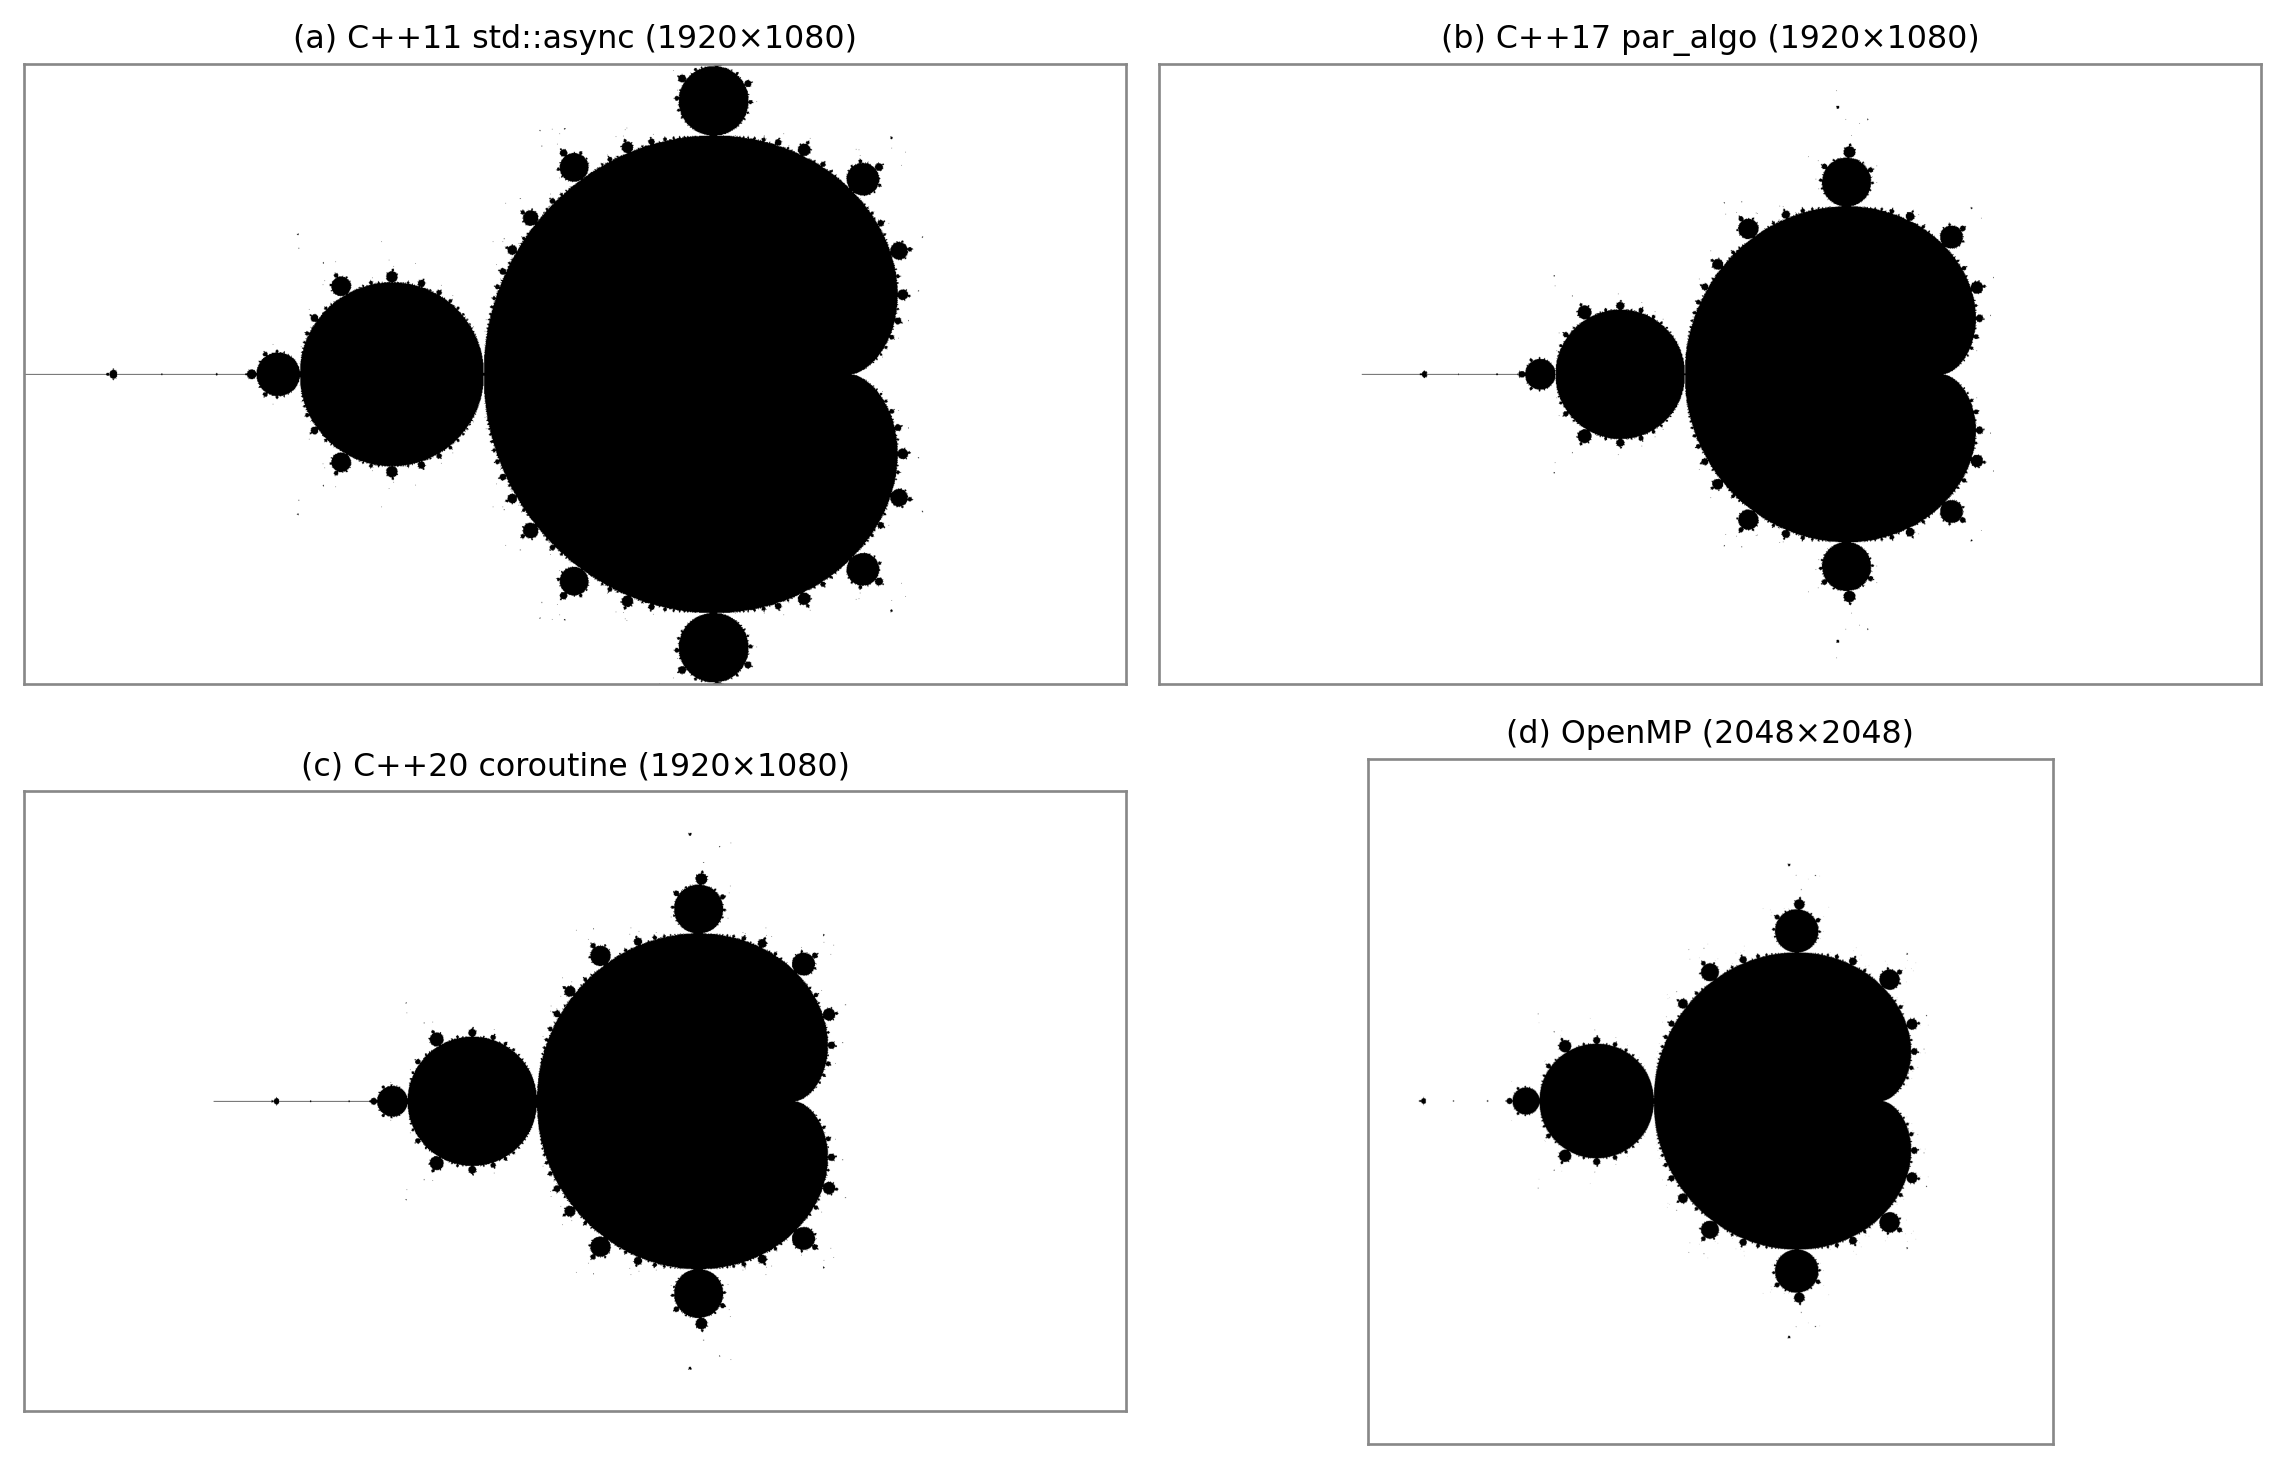
\includegraphics[width=0.92\textwidth]{figures/fig_gemini4_mandelbrot.png}
  \caption{Ảnh đầu ra định dạng P4 (chuyển sang PNG để hiển thị) do bốn biến thể
  bộ nhớ chia sẻ của Gemini 4 Hydrogen sinh ngay ở lần đầu: cả bốn đều đúng tỉ lệ
  hình học, rõ biên fractal và không gặp lỗi ảnh đen P4/P5.}
  \label{fig:gemini4mandel}
\end{figure}

\subsubsection{Khả năng mở rộng trên một nút và hàm ý rút ra}

Hình~\ref{fig:gemini4scaling} trình bày khả năng mở rộng trên một nút (12 luồng
logic) theo đúng hệ quy chiếu \emph{cập nhật điểm ảnh mỗi giây}
($\times 10^7$~px/s, Hình~\ref{fig:gemini4scaling}a) kèm đường tăng tốc tương đối
(Hình~\ref{fig:gemini4scaling}b), đối chiếu với mốc tham chiếu cục bộ
\code{mandel\_omp.cpp} ($0{,}51\to 5{,}36\times 10^7$~px/s, tăng tốc $10{,}55\times$).
Cả ba biến thể đa luồng của Gemini 4 Hydrogen đều tôn trọng tham số \code{-t}, có
độ dốc tuyến tính rõ rệt và không xuất hiện đường phẳng: OpenMP dẫn đầu về cả
thông lượng lẫn mức tăng tốc ($0{,}29\to 3{,}23\times 10^7$~px/s, $11{,}23\times$),
tiếp theo là C++20 coroutine ($0{,}18\to 1{,}85\times 10^7$~px/s, $10{,}50\times$)
và C++11 bất đồng bộ ($0{,}17\to 1{,}75\times 10^7$~px/s, $10{,}56\times$). Đáng
chú ý, quy đổi về \term{pixel updates per second} giúp loại bỏ sai lệch do khác
biệt độ phân giải mặc định: dù thời gian chạy của \code{openmp.cpp} ($0{,}130$~s ở
12 luồng) nhỉnh hơn \code{coroutine.cpp} ($0{,}112$~s), \code{openmp.cpp} xử lý
tới $2048\times 2048 = 4{,}19$~triệu điểm ảnh (gấp đôi $1920\times 1080$), nên đạt
thông lượng cao hơn gần $1{,}75\times$.

\begin{figure}[H]
  \centering
  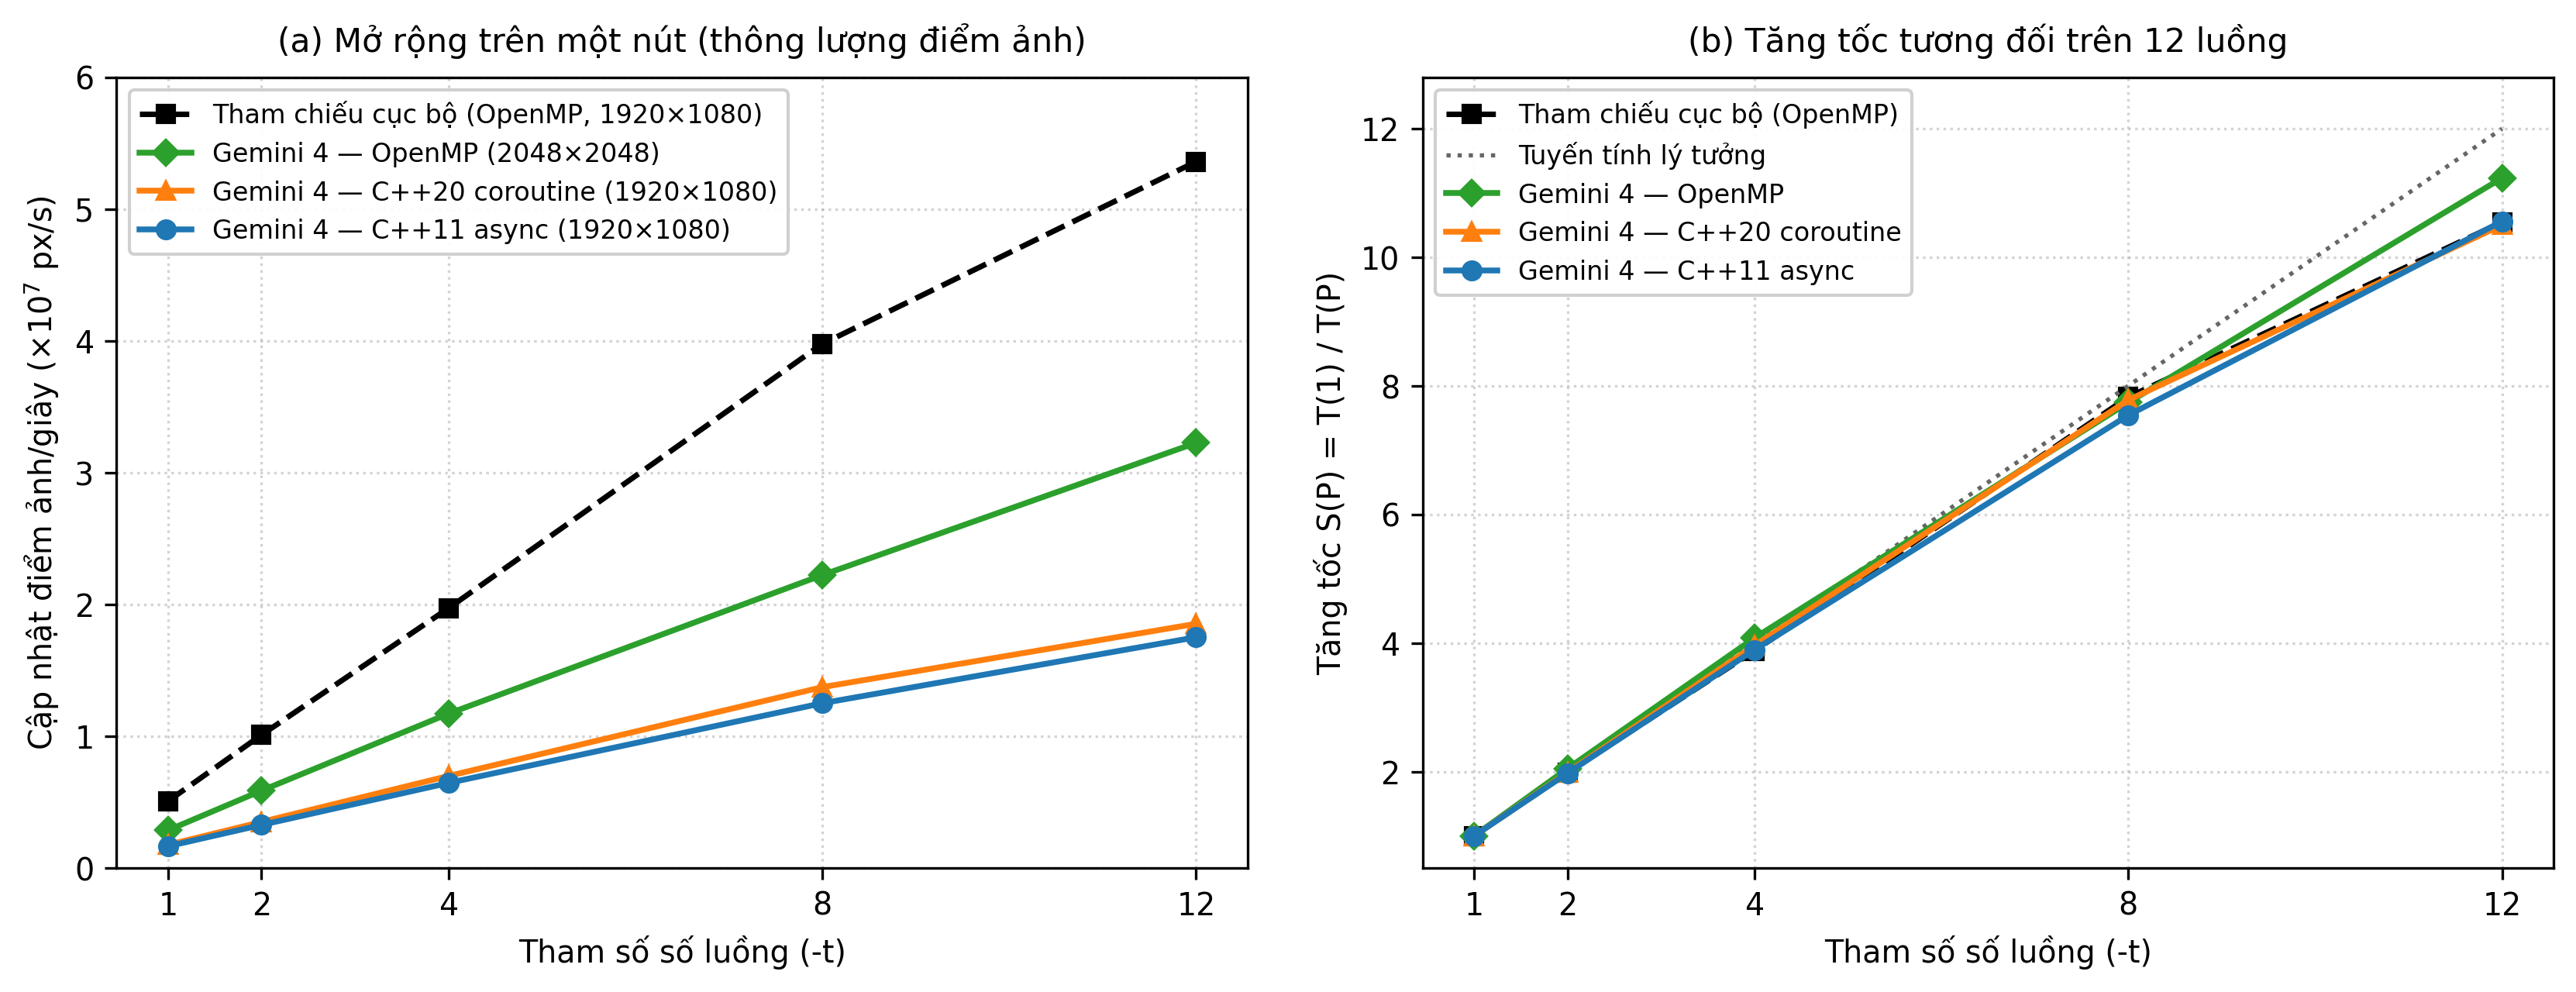
\includegraphics[width=0.98\textwidth]{figures/fig_gemini4_scaling.png}
  \caption{Khả năng mở rộng trên một nút của mã nguyên bản do Gemini 4 Hydrogen
  sinh (12 luồng cục bộ, trung bình 3 lần đo, loại trừ I/O) theo cùng hệ quy chiếu
  cập nhật điểm ảnh/giây ($\times 10^7$~px/s) với Hình~\ref{fig:scaling} và tăng
  tốc tương đối so với mốc tham chiếu \code{mandel\_omp.cpp}.}
  \label{fig:gemini4scaling}
\end{figure}

Ba nhận xét kỹ thuật rút ra từ thử nghiệm bổ sung này:

\begin{enumerate}
  \item \textbf{Khắc phục rõ rệt các lỗi cốt lõi của thế hệ trước.} Biến thể
        C++20 coroutine dùng \code{std::jthread} (đặt cuối danh sách thành viên để
        đảm bảo thứ tự hủy an toàn) kết hợp \code{std::latch}, tránh hoàn toàn lỗi
        treo vòng lặp \code{done()} của Claude và lỗi giải phóng hai lần của LLaMA.
        Biến thể C++17 kiểm tra sự tồn tại của \code{<tbb/global\_control.h>} bằng
        \code{\_\_has\_include} và cảnh báo tường minh khi thiếu backend thay vì
        đặt sai \code{OPENMP\_NUM\_THREADS}. Biến thể MPI+OpenMP chủ động dùng
        \code{MPI\_THREAD\_FUNNELED}, phân vùng \term{block-cyclic} theo \code{-p}
        (giảm rủi ro mất cân bằng tải ở bước $2\to 4$ nút) và gom dữ liệu bằng
        \code{MPI\_Gatherv} trước khi dừng \code{MPI\_Wtime()}.
  \item \textbf{Vẫn còn chi tiết nhỏ cần kiểm duyệt.} Ở \code{openmp.cpp}, mã gọi
        \code{std::fill} nhưng thiếu \code{\#include <algorithm>} tường minh (chỉ
        vượt qua trên GCC 13.2 nhờ kéo gián tiếp qua header chuẩn khác và có thể
        gặp lỗi trên trình biên dịch chặt hơn); đồng thời cờ cấu hình số vòng lặp
        không đồng nhất giữa các biến thể (\code{-i} ở \code{async}/\code{coroutine},
        \code{-m} ở \code{openmp}).
  \item \textbf{Độ nhạy của thông lượng tuyệt đối với đặc tả prompt.} Ngay cả khi
        đưa về cùng đơn vị cập nhật điểm ảnh/giây, độ cao tuyệt đối giữa các biến
        thể vẫn chênh lệch đáng kể: \code{async.cpp} và \code{coroutine.cpp} đạt
        $1{,}75\text{--}1{,}85\times 10^7$~px/s thấp hơn mốc tham chiếu
        ($5{,}36\times 10^7$~px/s) do miền tọa độ phức mặc định phóng sát hơn vào
        ruột tập Mandelbrot (tỉ lệ điểm chạm $I_{\max}$ cao hơn), trong khi
        \code{par\_algo.cpp} đạt tới $2{,}91\times 10^7$~px/s ngay trên một luồng
        nhờ tự bổ sung phép cắt tỉa hình tim và bóng chu kỳ 2. Điều này củng cố
        khuyến nghị ở Phần~\ref{sec:ketluan}: nếu muốn so sánh thông lượng tuyệt
        đối giữa các LLM, prompt cần cố định độ phân giải, miền tọa độ phức và
        tiêu chí tối ưu.
\end{enumerate}
